\documentclass[a4paper,12pt]{article}

\usepackage{amsmath}
\usepackage{amssymb}
\usepackage{algorithm}
\usepackage{algpseudocode}
\usepackage[backend=biber]{biblatex}
\usepackage{commath}
\usepackage{enumitem}
\usepackage{float}
\usepackage[a4paper,margin=25mm]{geometry}
\usepackage{graphicx}
\usepackage{mathtools}
\usepackage{tikz}
\usepackage{wrapfig}

\addbibresource{./main.bib}
\numberwithin{figure}{section}

\begin{document}

    \begin{titlepage}
    \centering
    {\LARGE Expanding the Concept of Geometric Inversion Beyond the $n$-Sphere\par}
    \vspace{2.0cm}
    {\Large Tarik Onalan \par}
    \vspace{1.0cm}
    {\Large \#\#\#\#\#\#--\#\#\#\# \par}
    \vspace{1.0cm}
    {\Large IB Mathematics HL \par}
    % \vfill
    % {\large Interlake High School\par}
    % \vspace{0.75cm}
    % {\large Vincent \textsc{Kessler}}
    \vfill
    {\Large May 2016}
\end{titlepage}
    
    \tableofcontents
    
    \section{Introduction}
    
        I am, by nature, a person who likes to question. I believe that understanding why certain bounds are set where they are is critical to operating optimally within those bounds.
        
        Thus, when I first heard about geometric inversion in one of my school's weekly math club meetings, I was questioning: ``Why is geometric inversion limited to circles?'' There seemed to me nothing precluding the inversion of points, lines, or shapes over, say, polygons. Yes, the radii of polygons are not constant around the centroid, but that did not seem to limit the possible application of geometric inversion to polygons. Even if the resulting transformation was not ``useful'', per se, it seemed to me an interesting exercise in geometry and linear algebra.
        
        Also, as a person who enjoys computer programming, geometric inversion seemed to be a problem space where programming could be useful, particularly in computing and visualizing geometric inverses. Thus, in order to aid with visualizing and manipulating inversions, I wrote a computer program that would automatically compute and plot the inversions of points, lines, and shapes.
        
        For this exploration, I will only consider the 1-sphere, commonly referred to as the circle, as visualization of geometric inversion in greater (or lesser) dimensions proved to be too difficult; however, the same operations and theorems that will be discussed in section \ref{sec:fun} still apply.
        
    \section{Fundamentals}\label{sec:fun}
    
        Geometric inversion is a transformation in Euclidean space. The geometric inverse of a point $P$ around an $n$-sphere in $\mathbb{R}^{n+1}$ centered at $O$ with radius $k$ is a point $P'$ such that:
        \[\abs{OP} \cdot \abs{OP'} = k^2\]
        \begin{figure}[H]
            \centering
            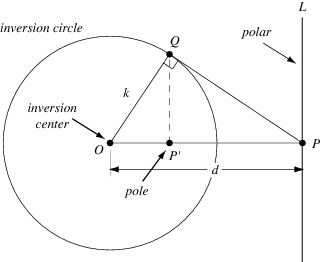
\includegraphics[scale=0.9]{./pictures/InversePoints}
            \caption{Basic geometric inversion}
            \label{fig:basic}
        \end{figure}
        
        Geometric inversion has certain properties that make it valuable for solving more advanced problems in geometry. The most important properties of geometric inversion are listed below, with visualizations of the properties:
        
        \begin{enumerate}[leftmargin=25mm,label=\textbf{Theorem \arabic*:}]
            \item The image of a line through a center of inversion $O$ is itself.
            \begin{figure}[H]
                \centering
                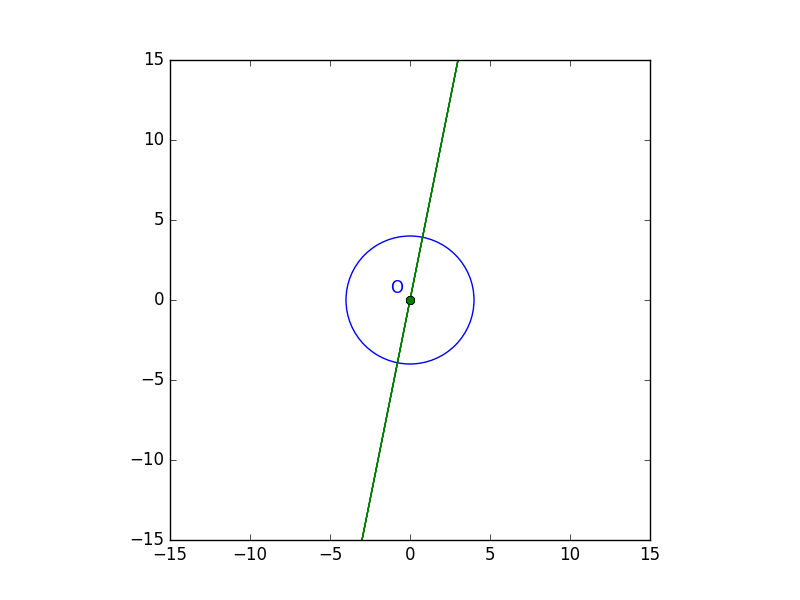
\includegraphics[scale=0.6]{./pictures/INVERT_LINE_CENTER}
                \caption{Inversion of the line $y=5x$ over the circle around $O$ yields itself}
                \label{fig:lcenter}
            \end{figure}
            \newpage
            \item The image under inversion of a line not passing through the center of inversion $O$ is a circle passing through the center of inversion $O$.
            \begin{figure}[H]
                \centering
                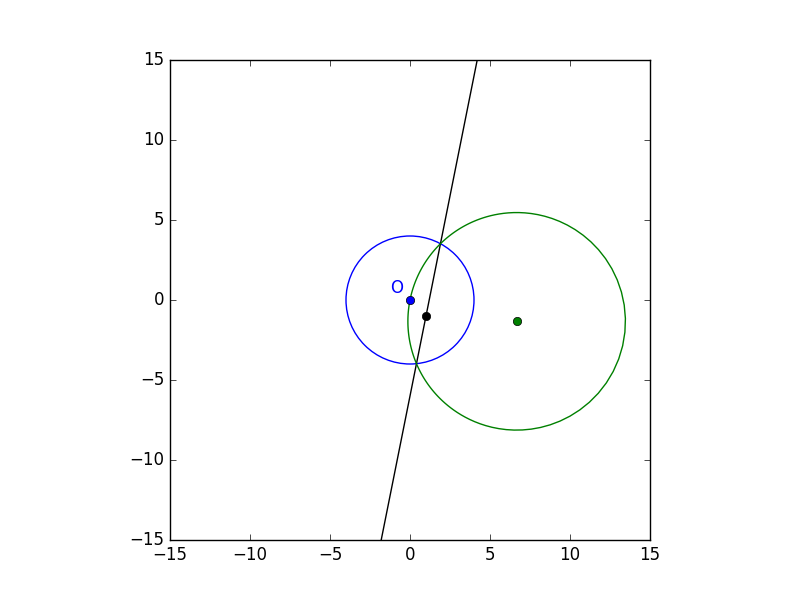
\includegraphics[scale=0.6]{./pictures/INVERT_LINE_OFFCENTER}
                \caption{Inversion of the line $y+1=5(x-1)$ over the circle around $O$ yields a circle through $O$.}
                \label{fig:loffcenter}
            \end{figure}
            \item The image under inversion of a circle not through the center of inversion is a circle.
            \begin{figure}[H]
                \centering
                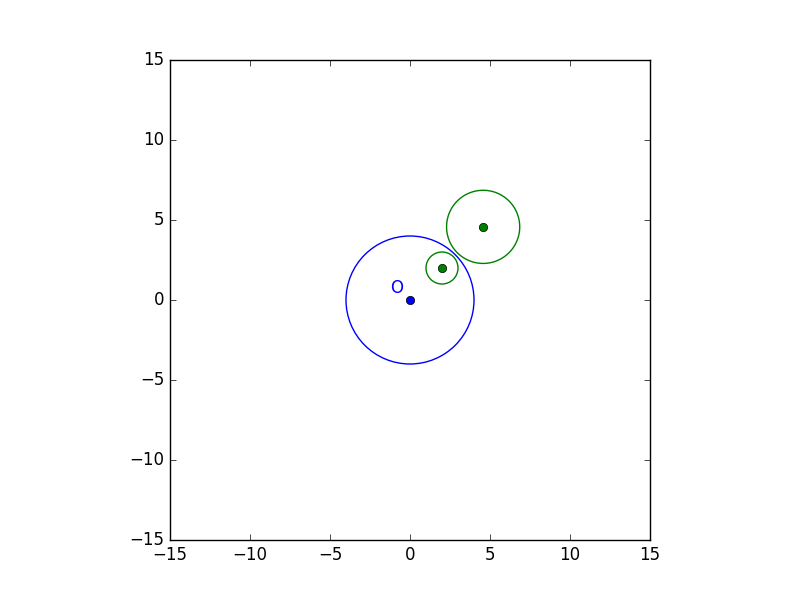
\includegraphics[scale=0.6]{./pictures/INVERT_CIRCLE_OFFCENTER}
                \caption{Inversion of the circle $(x-2)^2-(y-2)^2=1$ over the circle around $O$ yields another circle.}
                \label{fig:coffcenter}
            \end{figure}
            \newpage
            \item The magnitude of an angle between two intersecting curves is not changed by an inversion.
            \begin{figure}[H]
                \centering
                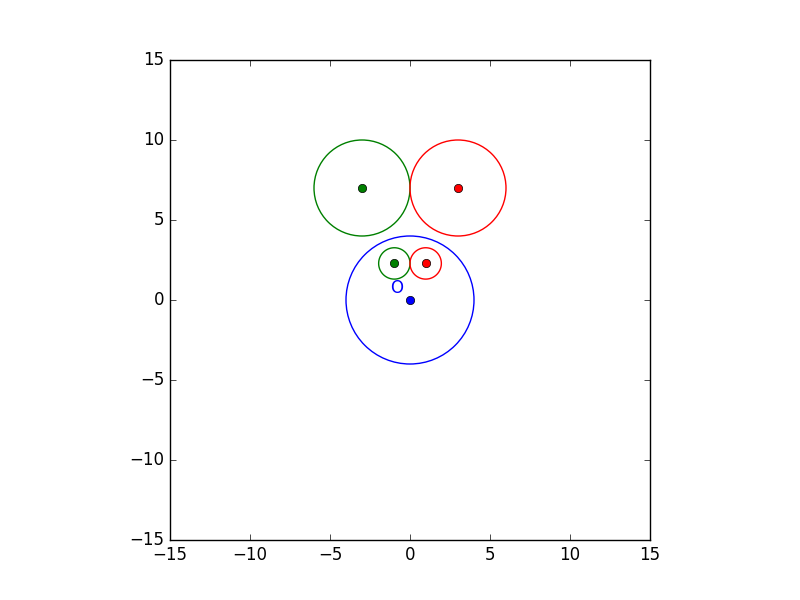
\includegraphics[scale=0.6]{./pictures/INVERT_CIRCLE_ANGLE}
                \caption{The tangential green and red circles outside of the circle around $O$ yield two tangential circles within the circle around $O$.}
                \label{fig:cangle}
            \end{figure}
            \item The image of a circle under inversion is itself if and only if the circle is orthogonal to the inversion circle.
            \begin{figure}[H]
                \centering
                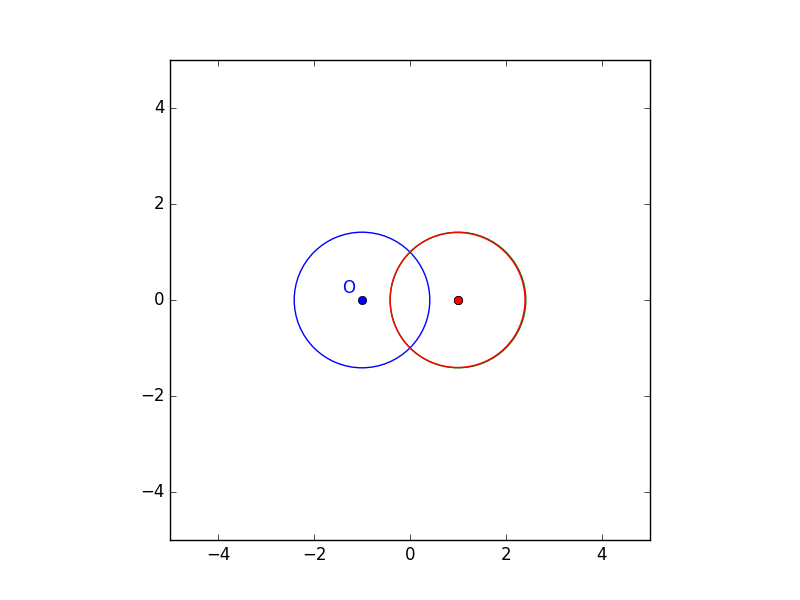
\includegraphics[scale=0.6]{./pictures/INVERT_CIRCLE_ORTHO}
                \caption{Inversion of a circle over an orthogonal circle around $O$ yields the same circle.}
                \label{fig:cortho}
            \end{figure}
        \end{enumerate}
        
    \section{The Shoemaker's Knife}
    
        The Shoemaker's Knife is a geometric problem very much suited towards using geometric inversion in its solution. Consider the following diagram:
        
        \begin{figure}[H]
            \centering
            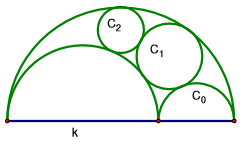
\includegraphics{./pictures/SHOEMAKER_KNIFE}
            \caption{The Shoemaker's Knife}
            \label{fig:knife}
        \end{figure}
        
        Three semicircles are mutually tangent on the line $k$, with circles $C_1$, $C_2$,... inscribed in the remaining space. The objective is to determine the height $h_n$ of circle $C_n$ is a distance $nd_n$ from line $k$, where $d_n$ is the diameter of circle $C_n$.
        
        The use of geometric inversion greatly eases the solution of this problem. We can label the large outer semicircle B, the smaller inner semicircle on the left A, and construct a circle orthogonal to $C_2$ $C$. Inverting over circle $C$ produces the following result:
        
        \begin{figure}[H]
            \centering
            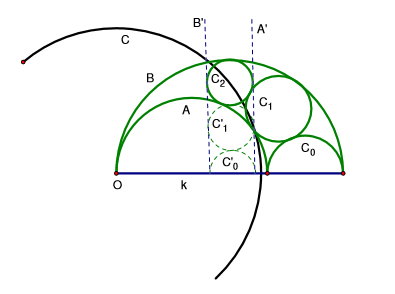
\includegraphics{./pictures/SHOEMAKER_KNIFE_INVERT}
            \caption{Inverting the Shoemaker's Knife over circle $C$}
            \label{fig:knifeinv}
        \end{figure}
        
        Using theorem 5, we know that $C_2$ maps to itself. Also, by theorem 2 and 4, respectively, we know that semicircles $A$ and $B$ map to straight lines perpendicular to $k$ and tangent to $C_2$. Thus, the diameter of circle $C_2$ is equal to the distance between lines $A'$ and $B'$.
        
        We must also consider the image of $C_1$ and $C_0$. Before inversion, $C_1$ was tangent to semicircles $A$ and $B$, so, by theorem 4, $C_1'$ is tangent to $A'$ and $B'$, and the diameter of $C_1'$ is equal to the distance between $A'$ and $B'$. This also applies to circle $C_0$ and its inverse, $C_0'$. Thus, we can now see that the height of the circle $C_2$ is equal to two times its diameter, proving that $h_n=nd_n$:
        
        \[h_2=\frac{d_2}{2}+d_1+\frac{d_0}{2}\]
        \[h_2=\frac{\abs{A'B'}}{2}+\abs{A'B'}+\frac{\abs{A'B'}}{2}\]
        \[h_2=2\abs{A'B'}\]
        
    \section{Extension Beyond the $n$-Sphere}
    
        Let me begin with an example of inversion over objects that are not $n$-spheres:
        
        \begin{figure}[H]
            \centering
            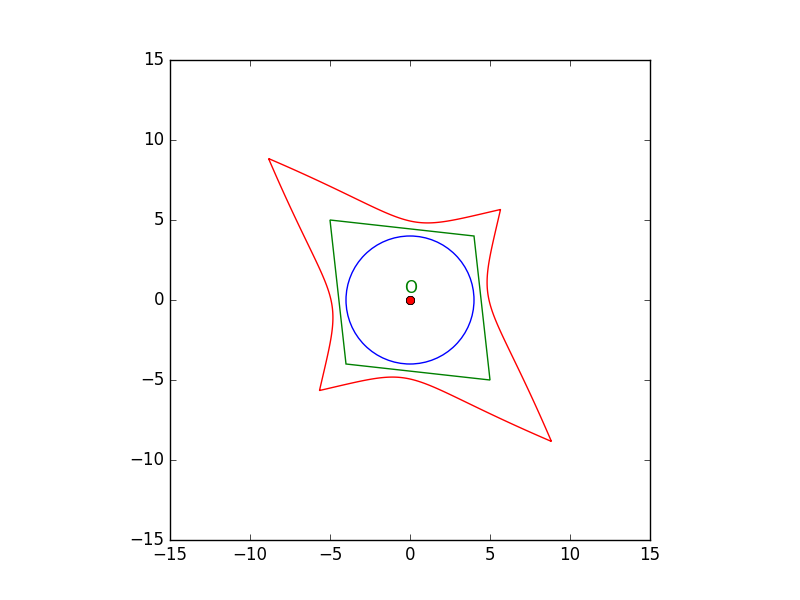
\includegraphics[scale=0.6]{./pictures/INVERT_CIRCLE_POLY}
            \caption{Inversion of the blue circle over the green polygon.}
            \label{fig:invcpoly}
        \end{figure}
        
        Note that inverting the green polygon over the blue circle does not yield the same result as inverting the blue circle over the green polygon (as shown below). This is because in the case where the blue circle is inverted over the green polygon, the radii are (besides constantly changing) consistently longer than the distance between the centroid of the polygon and any point along the arc of the circle. In the other case, where the green polygon is inverted over the circle, the distance from the inversion center to any point along the polygon is always longer than the radius of the circle.
        
        \begin{figure}[H]
            \centering
            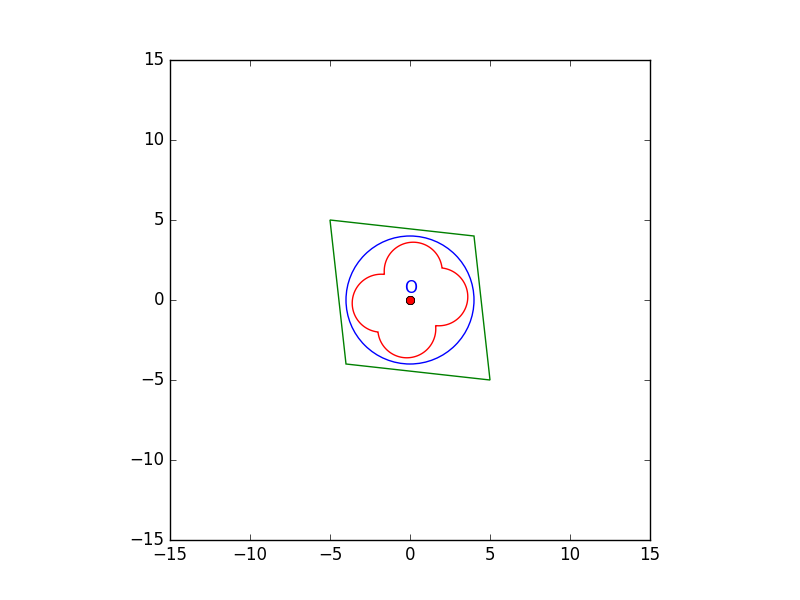
\includegraphics[scale=0.6]{./pictures/INVERT_POLY_CIRCLE}
            \caption{Inversion of the green polygon over the blue circle.}
            \label{fig:invpcircle}
        \end{figure}
        
        The math behind inverting over polygons was, to me, more complex than I had initially imagined. Things that could otherwise be trivial when done by hand, like measuring the nearest ``radii'' from the centroid of the polygon to the edge of the polygon, were surprisingly complex when written out by hand (and later, written in code).
        
        \begin{algorithm}[H]
            \caption{Get circle corresponding to external point.}
            \begin{algorithmic}
                \Function{GET\_CIRCLE}{vertices $vs$, centroid $c$, point $p$}
                    \State $dx \gets c_x - p_x$
                    \State $dy \gets c_y - p_y$
                    \State $m \gets \dfrac{dy}{dx}$
                    \Comment{Slope between centroid and external point}\\
                    \For{$i < \abs{vs}$}
                        \State $v1 \gets vs[i]$
                        \State $v2 \gets vs[(i+1) \bmod \abs{vs}]$
                        \Comment{Adjacent vertices of polygon}\\
                        
                        \State $dx_v \gets v1_x - v2_x$
                        \State $dy_v \gets v1_y - v2_y$
                        \State $m_v \gets \dfrac{dy_v}{dx_v}$
                        \Comment{Slope between vertices}\\
                        
                        \State $A \gets
                            \begin{pmatrix}
                                1 & -m\\
                                1 & -m_v
                            \end{pmatrix}$
                        \State $B \gets 
                            \begin{pmatrix}
                                m \cdot -c_x + c_y\\
                                m_v \cdot -v1_x + v1_y
                            \end{pmatrix}$
                        \Comment{From $y-y_0=m(x-x_0)$}
                        \State $X \gets A^{-1}B$
                        \Comment{Solve system of equations}\\
                        
                        \State $x \gets X_{2,1}$
                        \State $y \gets X_{1,1}$
                        \State $q \gets (x,y)$
                        \Comment{Extract solution from $X$}\\
                        
                        \If{$v1_x \leq q_x \leq v2_x$ and $v1_y \leq q_y \leq v2_y$}
                        \Comment{Check if $q$ is in range}
                            \If{$\text{arctan}\left(\dfrac{q_y-c_y}{q_x-c_x}\right)=\text{arctan}\left(m\right)$}
                            \Comment{Check for equal direction}
                                \State $r \gets \text{dist}\left(c,q\right)$
                                \Comment{Get radius from $c$ to $q$}
                                \State \Return $\text{Circle}\left(c,r\right)$
                                \Comment{Return circle at $c$ with radius $r$}
                            \EndIf
                        \EndIf
                    \EndFor
                \EndFunction
            \end{algorithmic}
        \end{algorithm}
        
        This procedure was the crux of inverting shapes over polygons. Being able to extract a circle corresponding to a point outside of the locus of points composing the polygon is central to carrying out the inversion step. After a circle is returned from the routine, the inversion operation proceeds as it does with a normal circle, though only for the specific point for which the circle was extracted. While this routine has been simplified both to fit in this paper and to remain comprehensible, the operations remain---for the most part---the same.
        
        \begin{figure}[H]
            \centering
            \begin{tikzpicture}
                \node[anchor=south west,inner sep=0] at (0,0) {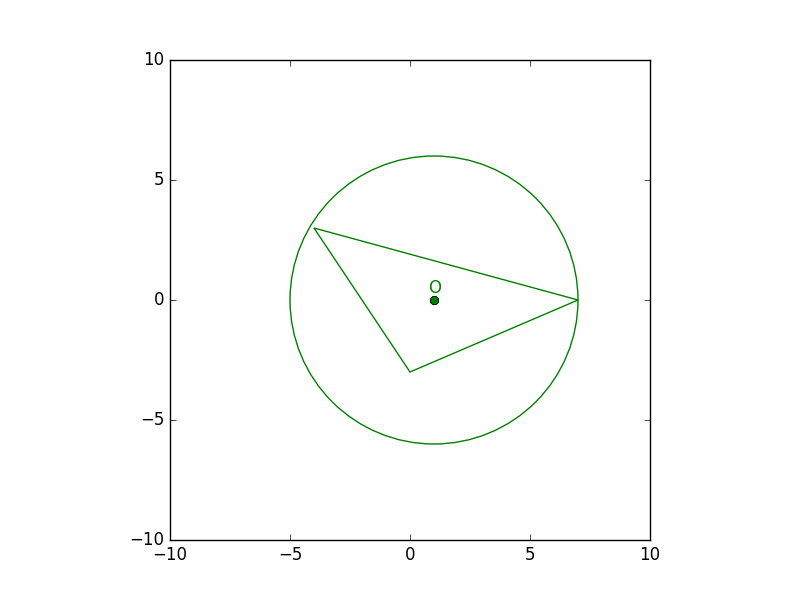
\includegraphics[scale=0.6]{./pictures/INVERT_SHOW_CIRCLES}};
                \filldraw[fill=red] (8.8,4.575) circle (3pt);
            \end{tikzpicture}
            \caption{Computed radius point (red) and circle (green, around $O$)}
            \label{fig:getcircle}
        \end{figure}
        
    \section{Extending Fundamentals}
    
        Now that we can invert over polygons, we can revisit the theorems that we discussed in section \ref{sec:fun}, checking to see how the theorems apply.
        
        \begin{enumerate}[leftmargin=25mm,label=\textbf{Theorem \arabic*:}]
            \item The image of a line through a center of inversion $O$ is itself.
                \begin{figure}[H]
                    \centering
                    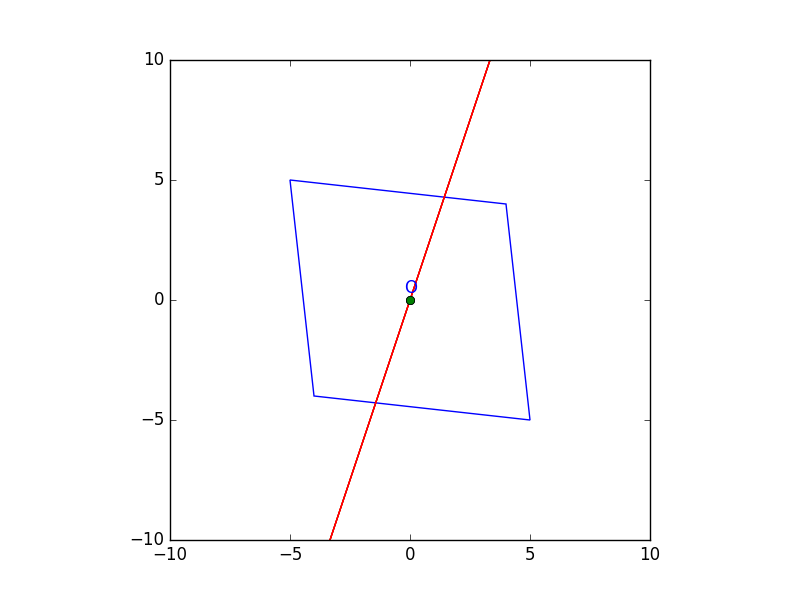
\includegraphics[scale=0.6]{./pictures/INVERT_LINE_POLY}
                    \caption{Inversion of the line $y=5x$ over the circle around $O$ yields itself.}
                    \label{fig:lpcenter}
                \end{figure}
            \item The image under inversion of a line not passing through the center of inversion $O$ is a closed curve through the center of inversion $O$.
            \begin{figure}[H]
                \centering                    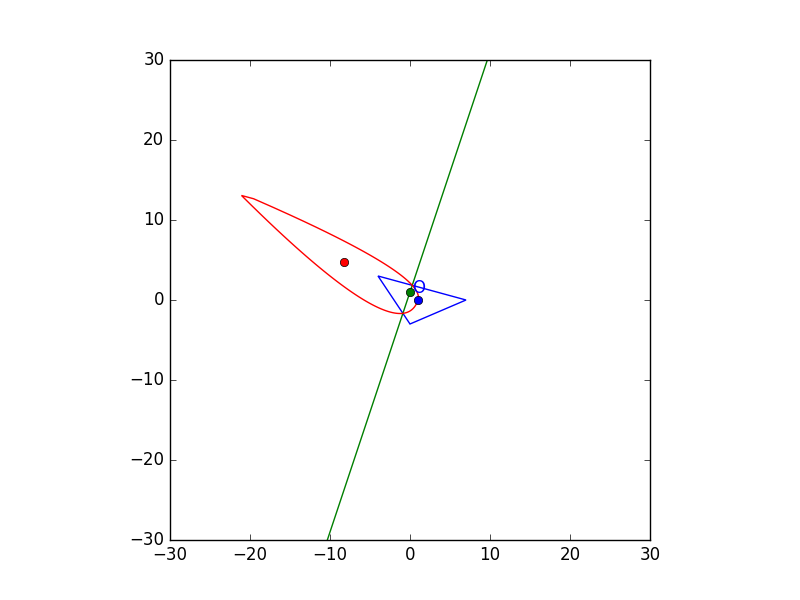
\includegraphics[scale=0.6]{./pictures/INVERT_LINEOFFC_POLY}
                \caption{Inversion of the line (green) over the polygon (blue) yields a plane curve (red) through the center of inversion $O$.}
                \label{fig:lpoffset}
            \end{figure}
            \item The image under inversion of a polygon not through the center of inversion is a closed curve not through the center of inversion.
            \begin{figure}[H]
                \centering                    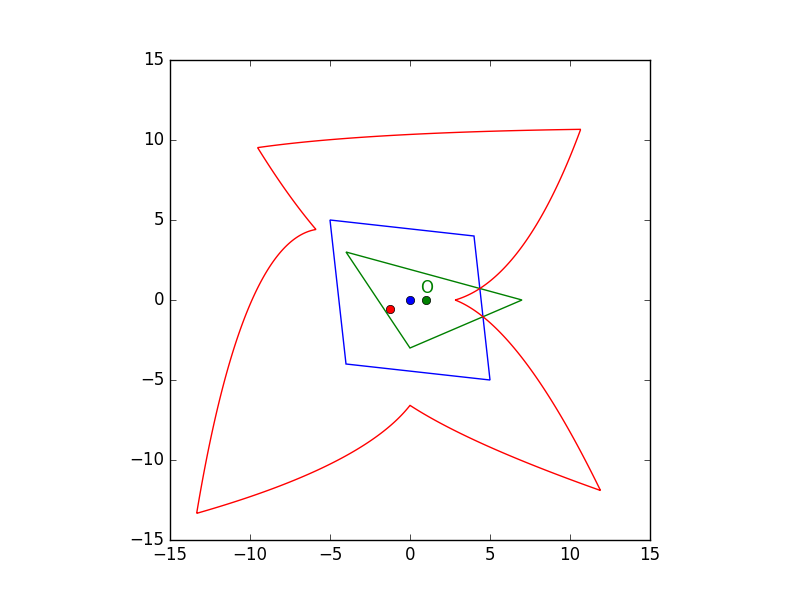
\includegraphics[scale=0.6]{./pictures/INVERT_POLYOFFC_POLY}
                \caption{Inversion of the triangle (green) over the quadrilateral (blue) yields a plane curve (red).}
                \label{fig:coffcenter}
            \end{figure}
        \end{enumerate}
        
        Unfortunately, I could not review theorems 4 and 5 due to limitations in my program.
            
    \section{Conclusion}
    
        Geometric inversion is a simple, yet powerful tool in geometric problem-solving. However, as I have demonstrated, it does not need to be limited to circles in its application. While my use of geometric inversion over polygons may not be as practically useful as inversion over circles, the intricacies of geometric inversion that I have learned while going about inverting over polygons has dramatically increased both my understanding and my appreciation of geometric inversion. On a final note, I would like to present the (near) infinite inversion of a polygon over another polygon, a circle, a polygon,...and a circle
        
        \begin{figure}[H]
            \centering
            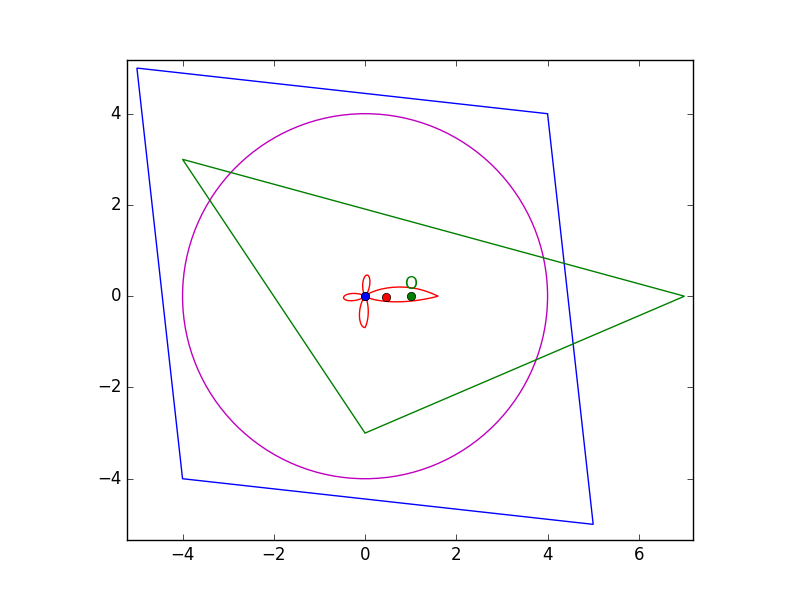
\includegraphics[scale=0.75]{./pictures/INVERT_POLYOFFC_POLY_INF}
            \caption{Infinite inversion}
            \label{fig:invmeta}
        \end{figure}
        
    \newpage
    
    \nocite{*}
    \printbibliography
\end{document}
